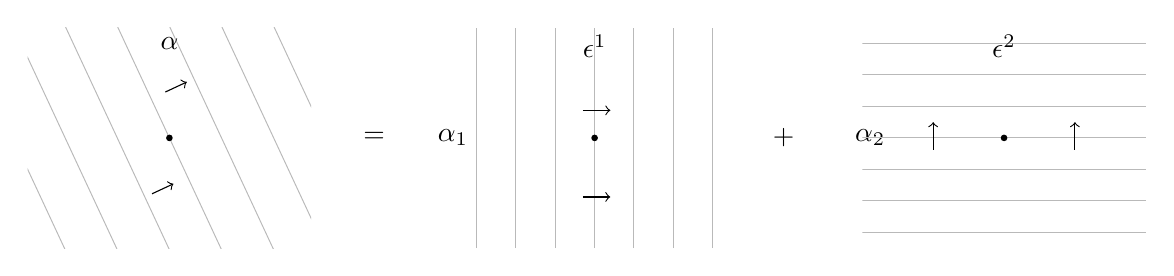
\begin{tikzpicture}[scale=1.0]
  % Layout anchors
  \node (A) at (0,0) {};

  % -------- left: alpha --------
  \begin{scope}[shift={(-5.2,0)}]
    \clip (-1.8,-1.4) rectangle (1.8,1.4);
    \begin{scope}[rotate=25]
      \foreach \x in {-3,-2.4,...,3} {
        \draw[gray!55, line width=0.35pt] (\x,-3) -- (\x,3);
      }
      \draw[->, black, line width=0.4pt] (-0.5,-0.55) -- (-0.2,-0.55);
      \draw[->, black, line width=0.4pt] (0.2,0.55) -- (0.5,0.55);
    \end{scope}
    \fill[black] (0,0) circle (1.2pt);
    \node[anchor=south] at (0,1.0) {$\alpha$};
  \end{scope}

  % -------- equals sign --------
  \node at (-2.6,0) {$=$};

  % -------- middle: alpha1 * epsilon1 --------
  \node at (-1.6,0) {$\alpha_1$};
  \begin{scope}[shift={(0.2,0)}]
    \clip (-1.8,-1.4) rectangle (1.8,1.4);
    \foreach \x in {-2,-1.5,...,2} {
      \draw[gray!55, line width=0.35pt] (\x,-1.4) -- (\x,1.4);
    }
    \draw[->, black, line width=0.4pt] (-0.15,-0.75) -- (0.2,-0.75);
    \draw[->, black, line width=0.4pt] (-0.15,0.35) -- (0.2,0.35);
    \fill[black] (0,0) circle (1.2pt);
    \node[anchor=south] at (0,0.9) {$\epsilon^1$};
  \end{scope}

  % -------- plus sign --------
  \node at (2.6,0) {$+$};

  % -------- right: alpha2 * epsilon2 --------
  \node at (3.7,0) {$\alpha_2$};
  \begin{scope}[shift={(5.4,0)}]
    \clip (-1.8,-1.4) rectangle (1.8,1.4);
    \foreach \y in {-1.2,-0.8,...,1.2} {
      \draw[gray!55, line width=0.35pt] (-1.8,\y) -- (1.8,\y);
    }
    \draw[->, black, line width=0.4pt] (-0.9,-0.15) -- (-0.9,0.2);
    \draw[->, black, line width=0.4pt] (0.9,-0.15) -- (0.9,0.2);
    \fill[black] (0,0) circle (1.2pt);
    \node[anchor=south] at (0,0.9) {$\epsilon^2$};
  \end{scope}
\end{tikzpicture}
